\documentclass[10pt]{article}
\usepackage[margin=0.8in]{geometry}
\usepackage[utf8]{inputenc}
\usepackage[T1]{fontenc}
\usepackage{graphicx}
\usepackage[export]{adjustbox}
\graphicspath{ {./lecture2-images/} }
\usepackage{amsmath}
\usepackage{amsfonts}
\usepackage{amssymb}
\usepackage[version=4]{mhchem}
\usepackage{stmaryrd}
\usepackage{bbold}
\usepackage{fixltx2e}
\usepackage{caption}
\usepackage{mathtools}
\usepackage[parfill]{parskip}
\usepackage{float}

\begin{document}



\title{Lecture 14: Statics and Duality}
\date{Oct. 5, 2023}
\author{Wanxin Jin}
\maketitle


\section{Statics}
Statics is to determine the relationship between the generalized forces applied to the end-effector and the generalized torques applied to the joints when the manipulator is at equilibrium. Let $\boldsymbol{\tau}$ be the $(n \times 1)$ joint torques and $\boldsymbol{\gamma}_{e}$ the $(r \times 1)$ end-effector forces. 
We will apply the principle of virtual work to determine this relationship. 

The elementary work by the joint torques:

$$
d W_{\tau}=\boldsymbol{\tau}^{T} d \boldsymbol{q}
$$



As for the end-effector forces  $\boldsymbol{\gamma}_{e}=\left[\boldsymbol{f}_{e}^{T} ,\boldsymbol{\mu}_{e}^{T}\right]^{T}$, including linear force $\boldsymbol{f}_{e}$ and moment  $\boldsymbol{\mu}_{e}$, the elementary work 

$$
d W_{\gamma}=\boldsymbol{f}_{e}^{T} d \boldsymbol{p}_{e}+\boldsymbol{\mu}_{e}^{T} \boldsymbol{\omega}_{e} d t =\boldsymbol{f}_{e}^{T} \boldsymbol{J}_{P}(\boldsymbol{q}) d \boldsymbol{q}+\boldsymbol{\mu}_{e}^{T} \boldsymbol{J}_{O}(\boldsymbol{q}) d \boldsymbol{q}  =\boldsymbol{\gamma}_{e}^{T} \boldsymbol{J}(\boldsymbol{q}) d \boldsymbol{q}
$$

where $d \boldsymbol{p}_{e}$ is the linear displacement and $\boldsymbol{\omega}_{e} d t$ is the angular displacement.

According to the principle of virtual work, the manipulator is at static equilibrium if and only if

$$
\delta W_{\tau}=\delta W_{\gamma} \quad \forall \delta \boldsymbol{q}
$$

This leads to



$$
\boldsymbol{\tau}=\boldsymbol{J}^{T}(\boldsymbol{q}) \boldsymbol{\gamma}_{e}
$$

stating a relationship between the end-effector forces and  joint torques, established by the transpose of the geometric Jacobian.

\section{Kineto-Statics Duality}




The kineto-statics duality states that

$$
\begin{aligned}
    \boldsymbol{v}_{e}=\boldsymbol{J}(\boldsymbol{q}) \dot{\boldsymbol{q}} \quad\quad\quad 
    \boldsymbol{\tau}=\boldsymbol{J}^{T}(\boldsymbol{q}) \boldsymbol{\gamma}_{e}
\end{aligned}
$$

\begin{itemize}
    \item The range space of $\boldsymbol{J}^{T}$ is the subspace $\mathcal{R}\left(\boldsymbol{J}^{T}\right)$ in $\mathbb{R}^{n}$ of the joint torques that can balance the end-effector forces,  given manipulator posture $\boldsymbol{q}$.

 \item The null space of $\boldsymbol{J}^{T}$ is the subspace $\mathcal{N}\left(\boldsymbol{J}^{T}\right)$ in $\mathbb{R}^{r}$ of the end-effector forces that do not require any balancing joint torques, given manipulator posture $\boldsymbol{q}$

\end{itemize}

\begin{figure}[H]
    \centering
    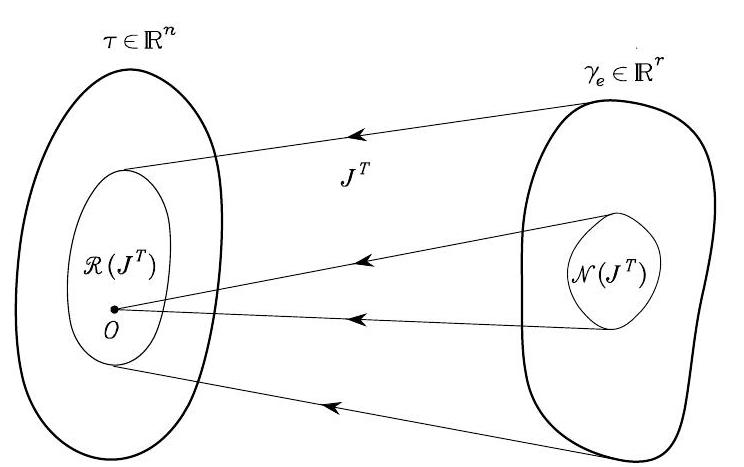
\includegraphics[max width=0.45\textwidth]{diff_kinematics/operation_to_joint.jpg}
    \caption{Mapping between the end-effector force space and the joint torque space}
    \label{fig:enter-label}
\end{figure}




It is worth remarking that the end-effector forces $\gamma_{e} \in \mathcal{N}\left(\boldsymbol{J}^{T}\right)$ are entirely absorbed by the structure in that the mechanical constraint reaction forces can balance them exactly. Hence, a manipulator at a singular configuration remains in the given posture whatever end-effector force $\gamma_{e}$ is applied so that $\gamma_{e} \in \mathcal{N}\left(J^{T}\right)$

The relations between the two subspaces are established by

$$
\mathcal{N}(\boldsymbol{J}) \equiv \mathcal{R}^{\perp}\left(\boldsymbol{J}^{T}\right) \quad \mathcal{R}(\boldsymbol{J}) \equiv \mathcal{N}^{\perp}\left(\boldsymbol{J}^{T}\right)
$$

and then, once the manipulator Jacobian is known, it is possible to characterize completely differential kinematics and statics in terms of the range and null spaces of the Jacobian and its transpose.


\section{Velocity and Force Transformation}

\begin{figure}[H]
    \centering
    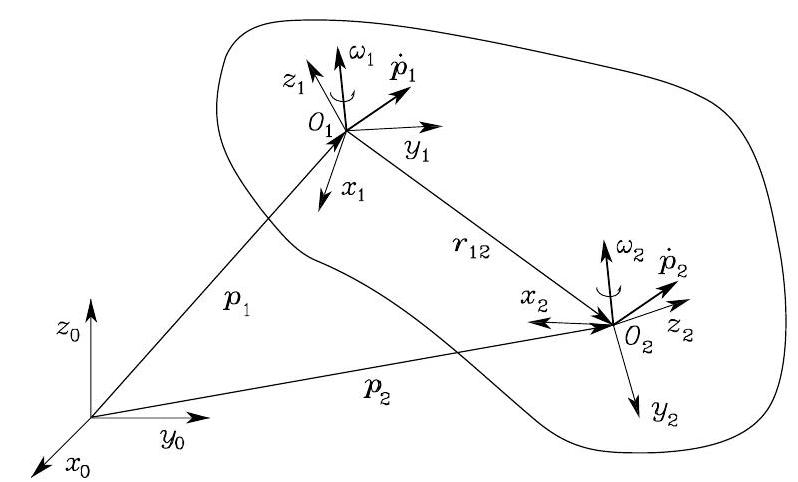
\includegraphics[max width=0.5\textwidth]{diff_kinematics/coordinate_mapping.jpg}
    \caption{Representation of linear and angular velocities in different coordinate frames on the same rigid body}
    \label{fig:enter-label}
\end{figure}


The kineto-statics duality concept presented above can be useful to characterize the transformation of velocities and forces between two coordinate frames. Consider a reference coordinate frame $O_{0}-x_{0} y_{0} z_{0}$ and a rigid body moving with respect to such a frame. Then let $O_{1}-x_{1} y_{1} z_{1}$ and $O_{2}-x_{2} y_{2} z_{2}$ be two coordinate frames attached to the body. The relationships between translational and rotational velocities of the two frames with respect to the reference frame are given by

$$
\begin{aligned}
\boldsymbol{\omega}_{2} & =\boldsymbol{\omega}_{1} \\
\dot{\boldsymbol{p}}_{2} & =\dot{\boldsymbol{p}}_{1}+\boldsymbol{\omega}_{1} \times \boldsymbol{r}_{12} .
\end{aligned}
$$

The above relations can be compactly written as

$$
\left[\begin{array}{c}
\dot{\boldsymbol{p}}_{2} \\
\boldsymbol{\omega}_{2}
\end{array}\right]=\left[\begin{array}{cc}
\boldsymbol{I} & -\boldsymbol{S}\left(\boldsymbol{r}_{12}\right) \\
\boldsymbol{O} & \boldsymbol{I}
\end{array}\right]\left[\begin{array}{c}
\dot{\boldsymbol{p}}_{1} \\
\boldsymbol{\omega}_{1}
\end{array}\right]
$$

On the other hand, if vectors are referred to their own frames, it is

$$
\left[\begin{array}{c}
\dot{\boldsymbol{p}}_{2}^{2} \\
\boldsymbol{\omega}_{2}^{2}
\end{array}\right]=\left[\begin{array}{cc}
\boldsymbol{R}_{1}^{2} & -\boldsymbol{R}_{1}^{2} \boldsymbol{S}\left(\boldsymbol{r}_{12}^{1}\right) \\
\boldsymbol{O} & \boldsymbol{R}_{1}^{2}
\end{array}\right]\left[\begin{array}{c}
\dot{\boldsymbol{p}}_{1}^{1} \\
\boldsymbol{\omega}_{1}^{1}
\end{array}\right]
$$



giving the  relationship of velocity transformation between two frames. The above can be compactly written as



$$
\boldsymbol{v}_{2}^{2}=\boldsymbol{J}_{1}^{2} \boldsymbol{v}_{1}^{1}
$$

By virtue of the kineto-statics duality, the force transformation between two frames is

$$
\boldsymbol{\gamma}_{1}^{1}=\boldsymbol{J}_{1}^{2 T} \boldsymbol{\gamma}_{2}^{2}
$$



Finally, notice that the above analysis is instantaneous in that, if a coordinate frame varies with respect to the other, it is necessary to recompute the Jacobian of the transformation through the computation of the related rotation matrix of one frame with respect to the other.




\end{document}